\documentclass{book}
\usepackage[a4paper,top=2.5cm,bottom=2.5cm,left=2.5cm,right=2.5cm]{geometry}
\usepackage{makeidx}
\usepackage{natbib}
\usepackage{graphicx}
\usepackage{multicol}
\usepackage{float}
\usepackage{listings}
\usepackage{color}
\usepackage{ifthen}
\usepackage[table]{xcolor}
\usepackage{textcomp}
\usepackage{alltt}
\usepackage[utf8]{inputenc}
\usepackage{mathptmx}
\usepackage[scaled=.90]{helvet}
\usepackage{courier}
\usepackage{sectsty}
\usepackage[titles]{tocloft}
\usepackage{doxygen}
\lstset{language=C++,inputencoding=utf8,basicstyle=\footnotesize,breaklines=true,breakatwhitespace=true,tabsize=4,numbers=left }
\makeindex
\setcounter{tocdepth}{3}
\renewcommand{\footrulewidth}{0.4pt}
\renewcommand{\familydefault}{\sfdefault}
\hfuzz=15pt
\setlength{\emergencystretch}{15pt}
\hbadness=750
\tolerance=750
\begin{document}
\begin{titlepage}
\vspace*{7cm}
\begin{center}
{\Large Phil\-Robokit Coding Guidelines }\\
\vspace*{1cm}
{\large Generated by Doxygen 1.8.1.1}\\
\vspace*{0.5cm}
{\small Tue Jul 17 2012 00:05:42}\\
\end{center}
\end{titlepage}
\clearemptydoublepage
\pagenumbering{roman}
\tableofcontents
\clearemptydoublepage
\pagenumbering{arabic}
\chapter{File Index}
\section{File List}
Here is a list of all files with brief descriptions\-:\begin{DoxyCompactList}
\item\contentsline{section}{{\bf Analog\-Output.\-phr} }{\pageref{_analog_output_8phr}}{}
\item\contentsline{section}{{\bf Blink\-Without\-Delay.\-phr} }{\pageref{_blink_without_delay_8phr}}{}
\item\contentsline{section}{{\bf corelib\-\_\-8bit\-\_\-timer.\-c} }{\pageref{corelib__8bit__timer_8c}}{}
\item\contentsline{section}{{\bf corelib\-\_\-8bit\-\_\-timer.\-h} }{\pageref{corelib__8bit__timer_8h}}{}
\item\contentsline{section}{{\bf corelib\-\_\-adc.\-c} }{\pageref{corelib__adc_8c}}{}
\item\contentsline{section}{{\bf corelib\-\_\-adc.\-h} }{\pageref{corelib__adc_8h}}{}
\item\contentsline{section}{{\bf corelib\-\_\-pwm.\-c} }{\pageref{corelib__pwm_8c}}{}
\item\contentsline{section}{{\bf corelib\-\_\-pwm.\-h} }{\pageref{corelib__pwm_8h}}{}
\item\contentsline{section}{{\bf corelib\-\_\-timer.\-c} }{\pageref{corelib__timer_8c}}{}
\item\contentsline{section}{{\bf corelib\-\_\-timer.\-h} }{\pageref{corelib__timer_8h}}{}
\item\contentsline{section}{{\bf corelib\-\_\-uart.\-c} }{\pageref{corelib__uart_8c}}{}
\item\contentsline{section}{{\bf corelib\-\_\-uart.\-h} }{\pageref{corelib__uart_8h}}{}
\item\contentsline{section}{{\bf corelib\-\_\-user\-\_\-interrupt.\-c} }{\pageref{corelib__user__interrupt_8c}}{}
\item\contentsline{section}{{\bf corelib\-\_\-user\-\_\-interrupt.\-h} }{\pageref{corelib__user__interrupt_8h}}{}
\item\contentsline{section}{{\bf htc\-\_\-16f87xa.\-h} }{\pageref{htc__16f87xa_8h}}{}
\item\contentsline{section}{{\bf htc\-\_\-16f87xa\-\_\-\-S\-P\-Lint.\-h} }{\pageref{htc__16f87xa___s_p_lint_8h}}{}
\item\contentsline{section}{{\bf htc\-\_\-common.\-h} }{\pageref{htc__common_8h}}{}
\item\contentsline{section}{{\bf htc\-\_\-common\-\_\-\-S\-P\-Lint.\-h} }{\pageref{htc__common___s_p_lint_8h}}{}
\item\contentsline{section}{{\bf i2c.\-c} }{\pageref{i2c_8c}}{}
\item\contentsline{section}{{\bf i2c.\-h} }{\pageref{i2c_8h}}{}
\item\contentsline{section}{{\bf Multiple\-Servos.\-phr} }{\pageref{_multiple_servos_8phr}}{}
\item\contentsline{section}{{\bf Phil\-Robo\-Kit\-\_\-\-Core\-Lib\-\_\-\-Data\-Types.\-h} }{\pageref{_phil_robo_kit___core_lib___data_types_8h}}{}
\item\contentsline{section}{{\bf Phil\-Robokit\-\_\-\-Core\-Lib\-\_\-\-Global\-Defs.\-c} }{\pageref{_phil_robokit___core_lib___global_defs_8c}}{}
\item\contentsline{section}{{\bf Phil\-Robo\-Kit\-\_\-\-Core\-Lib\-\_\-\-Header.\-h} }{\pageref{_phil_robo_kit___core_lib___header_8h}}{}
\item\contentsline{section}{{\bf Phil\-Robo\-Kit\-\_\-\-Core\-Lib\-\_\-\-Macro.\-c} }{\pageref{_phil_robo_kit___core_lib___macro_8c}}{}
\item\contentsline{section}{{\bf Phil\-Robo\-Kit\-\_\-\-Core\-Lib\-\_\-\-Macro.\-h} }{\pageref{_phil_robo_kit___core_lib___macro_8h}}{}
\item\contentsline{section}{{\bf P\-P\-M\-Generator.\-phr} }{\pageref{_p_p_m_generator_8phr}}{}
\item\contentsline{section}{{\bf P\-W\-M.\-phr} }{\pageref{_p_w_m_8phr}}{}
\item\contentsline{section}{{\bf servo.\-c} }{\pageref{servo_8c}}{}
\item\contentsline{section}{{\bf servo.\-h} }{\pageref{servo_8h}}{}
\item\contentsline{section}{{\bf Servo\-Port.\-phr} }{\pageref{_servo_port_8phr}}{}
\item\contentsline{section}{{\bf Servos.\-phr} }{\pageref{_servos_8phr}}{}
\item\contentsline{section}{{\bf spi.\-c} }{\pageref{spi_8c}}{}
\item\contentsline{section}{{\bf spi.\-h} }{\pageref{spi_8h}}{}
\item\contentsline{section}{{\bf User\-Interrupt.\-phr} }{\pageref{_user_interrupt_8phr}}{}
\end{DoxyCompactList}

\chapter{File Documentation}
\section{\-\_\-\-\_\-lib\-\_\-template.\-c File Reference}
\label{____lib__template_8c}\index{\-\_\-\-\_\-lib\-\_\-template.\-c@{\-\_\-\-\_\-lib\-\_\-template.\-c}}
{\ttfamily \#include \char`\"{}\-\_\-\-\_\-lib\-\_\-template.\-h\char`\"{}}\\*
Include dependency graph for \-\_\-\-\_\-lib\-\_\-template.\-c\-:\nopagebreak
\begin{figure}[H]
\begin{center}
\leavevmode
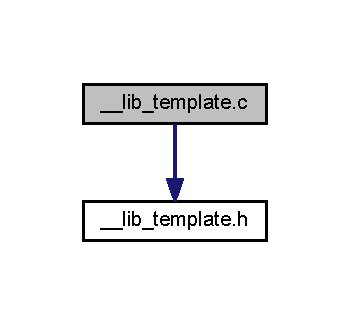
\includegraphics[width=168pt]{____lib__template_8c__incl}
\end{center}
\end{figure}
\subsection*{Macros}
\begin{DoxyCompactItemize}
\item 
\#define {\bf \-\_\-\-\_\-\-M\-O\-D\-U\-L\-E\-\_\-\-H\-E\-A\-D\-E\-R\-\_\-\-\_\-}
\begin{DoxyCompactList}\small\item\em This section was added for the Module Header to be shown on the documentation. \end{DoxyCompactList}\item 
\#define {\bf K8\-\_\-\-C\-O\-N\-S\-T\-A\-N\-T\-S}~3\-U\-C
\begin{DoxyCompactList}\small\item\em Constants (Local or Global) \end{DoxyCompactList}\end{DoxyCompactItemize}
\subsection*{Functions}
\begin{DoxyCompactItemize}
\item 
void {\bf call\-Public\-Functions} ()
\begin{DoxyCompactList}\small\item\em Public Functions are functions that are accessible outside the module. \end{DoxyCompactList}\item 
uint8\-\_\-t {\bf show\-Formula} (uint8\-\_\-t ui8\-X\-\_\-\-Value)
\begin{DoxyCompactList}\small\item\em Formula can also be documented by enclosing it between \textbackslash{}f\$ symbol. \end{DoxyCompactList}\item 
void {\bf main} (void)
\begin{DoxyCompactList}\small\item\em Contains a brief description of what a function does. This brief description can span multiple lines and is terminated by an empty line. \end{DoxyCompactList}\end{DoxyCompactItemize}


\subsection{Macro Definition Documentation}
\index{\-\_\-\-\_\-lib\-\_\-template.\-c@{\-\_\-\-\_\-lib\-\_\-template.\-c}!\-\_\-\-\_\-\-M\-O\-D\-U\-L\-E\-\_\-\-H\-E\-A\-D\-E\-R\-\_\-\-\_\-@{\-\_\-\-\_\-\-M\-O\-D\-U\-L\-E\-\_\-\-H\-E\-A\-D\-E\-R\-\_\-\-\_\-}}
\index{\-\_\-\-\_\-\-M\-O\-D\-U\-L\-E\-\_\-\-H\-E\-A\-D\-E\-R\-\_\-\-\_\-@{\-\_\-\-\_\-\-M\-O\-D\-U\-L\-E\-\_\-\-H\-E\-A\-D\-E\-R\-\_\-\-\_\-}!__lib_template.c@{\-\_\-\-\_\-lib\-\_\-template.\-c}}
\subsubsection[{\-\_\-\-\_\-\-M\-O\-D\-U\-L\-E\-\_\-\-H\-E\-A\-D\-E\-R\-\_\-\-\_\-}]{\setlength{\rightskip}{0pt plus 5cm}\#define \-\_\-\-\_\-\-M\-O\-D\-U\-L\-E\-\_\-\-H\-E\-A\-D\-E\-R\-\_\-\-\_\-}\label{____lib__template_8c_af75326f3ca42905e32d07f10c31e78fb}


This section was added for the Module Header to be shown on the documentation. 

\subsection*{Phil\-Robotics $|$ Philippine Electronics and Robotics Enthusiasts Club}

{\tt http\-://philrobotics.\-com} $|$ {\tt http\-://philrobotics.\-com/forum} $|$ {\tt http\-://facebook.\-com/philrobotics} {\tt phirobotics.\-core@philrobotics.\-com} 

 \begin{TabularC}{2}
\hline
\rowcolor{lightgray}{\bf Filename\-: }&{\bf \char`\"{}\-\_\-\-\_\-lib\-\_\-template.\-c\char`\"{} }\\\cline{1-2}
Description\-: &This is a coding standard template file \\\cline{1-2}
Revision\-: &v00.\-00.\-01 \\\cline{1-2}
Author\-: &Efren S. Cruzat I\-I \\\cline{1-2}
&\\\cline{1-2}
Dependencies\-:&\\\cline{1-2}
\end{TabularC}


\begin{quotation}
This program is free software\-: you can redistribute it and/or modify it under the terms of the G\-N\-U General Public License as published by the Free Software Foundation, either version 3 of the License, or (at your option) any later version. This program is distributed in the hope that it will be useful, but W\-I\-T\-H\-O\-U\-T A\-N\-Y W\-A\-R\-R\-A\-N\-T\-Y; without even the implied warranty of M\-E\-R\-C\-H\-A\-N\-T\-A\-B\-I\-L\-I\-T\-Y or F\-I\-T\-N\-E\-S\-S F\-O\-R A P\-A\-R\-T\-I\-C\-U\-L\-A\-R P\-U\-R\-P\-O\-S\-E. See the G\-N\-U General Public License for more details. \par
\par
 You should have received a copy of the G\-N\-U General Public License along with this program. If not, see {\tt http\-://www.\-gnu.\-org/licenses/}

\end{quotation}


 \begin{TabularC}{4}
\hline
\rowcolor{lightgray}{\bf F\-W Version }&{\bf Date }&{\bf Author }&{\bf Description }\\\cline{1-4}
v00.\-00.\-01 &20120714 &E\-S\-C\-I\-I &Library Initial Release \\\cline{1-4}
\end{TabularC}


Definition at line 32 of file \-\_\-\-\_\-lib\-\_\-template.\-c.

\index{\-\_\-\-\_\-lib\-\_\-template.\-c@{\-\_\-\-\_\-lib\-\_\-template.\-c}!K8\-\_\-\-C\-O\-N\-S\-T\-A\-N\-T\-S@{K8\-\_\-\-C\-O\-N\-S\-T\-A\-N\-T\-S}}
\index{K8\-\_\-\-C\-O\-N\-S\-T\-A\-N\-T\-S@{K8\-\_\-\-C\-O\-N\-S\-T\-A\-N\-T\-S}!__lib_template.c@{\-\_\-\-\_\-lib\-\_\-template.\-c}}
\subsubsection[{K8\-\_\-\-C\-O\-N\-S\-T\-A\-N\-T\-S}]{\setlength{\rightskip}{0pt plus 5cm}\#define K8\-\_\-\-C\-O\-N\-S\-T\-A\-N\-T\-S~3\-U\-C}\label{____lib__template_8c_a28927887322c9fa75b2aebd172f28e38}


Constants (Local or Global) 


\begin{DoxyItemize}
\item + must have prefixed with \char`\"{}\-K$<$\#of\-\_\-bits$>$\-\_\-\char`\"{}
\begin{DoxyItemize}
\item must be written on all caps
\item value must have explicitly defined type 
\end{DoxyItemize}
\end{DoxyItemize}

Definition at line 38 of file \-\_\-\-\_\-lib\-\_\-template.\-c.



\subsection{Function Documentation}
\index{\-\_\-\-\_\-lib\-\_\-template.\-c@{\-\_\-\-\_\-lib\-\_\-template.\-c}!call\-Public\-Functions@{call\-Public\-Functions}}
\index{call\-Public\-Functions@{call\-Public\-Functions}!__lib_template.c@{\-\_\-\-\_\-lib\-\_\-template.\-c}}
\subsubsection[{call\-Public\-Functions}]{\setlength{\rightskip}{0pt plus 5cm}void call\-Public\-Functions (
\begin{DoxyParamCaption}
{}
\end{DoxyParamCaption}
)}\label{____lib__template_8c_a3a6923995f4e3e60ca42cfd6c1b9849b}


Public Functions are functions that are accessible outside the module. 


\begin{DoxyItemize}
\item function name must follow the format $<$action$>$$<$\-Module$>$$<$\-Parameter$>$
\begin{DoxyItemize}
\item e.\-g. get\-Pin\-Value(\-Pin)
\end{DoxyItemize}
\item A prototype of the function must always be defined at the .h file of that module
\item If a function has no parameter the \char`\"{}void\char`\"{} type is omitted to prevent Hi-\/\-Tech C warnings 
\end{DoxyItemize}$<$ Variables local to a function must have assigned values before it can be used 

Definition at line 69 of file \-\_\-\-\_\-lib\-\_\-template.\-c.

\index{\-\_\-\-\_\-lib\-\_\-template.\-c@{\-\_\-\-\_\-lib\-\_\-template.\-c}!main@{main}}
\index{main@{main}!__lib_template.c@{\-\_\-\-\_\-lib\-\_\-template.\-c}}
\subsubsection[{main}]{\setlength{\rightskip}{0pt plus 5cm}void main (
\begin{DoxyParamCaption}
\item[{void}]{}
\end{DoxyParamCaption}
)}\label{____lib__template_8c_a6288eba0f8e8ad3ab1544ad731eb7667}


Contains a brief description of what a function does. This brief description can span multiple lines and is terminated by an empty line. 

Detailed Description can start after the empty line. Entries entered on the detailed description are not shown on the summary view 

Definition at line 99 of file \-\_\-\-\_\-lib\-\_\-template.\-c.

\index{\-\_\-\-\_\-lib\-\_\-template.\-c@{\-\_\-\-\_\-lib\-\_\-template.\-c}!show\-Formula@{show\-Formula}}
\index{show\-Formula@{show\-Formula}!__lib_template.c@{\-\_\-\-\_\-lib\-\_\-template.\-c}}
\subsubsection[{show\-Formula}]{\setlength{\rightskip}{0pt plus 5cm}uint8\-\_\-t show\-Formula (
\begin{DoxyParamCaption}
\item[{uint8\-\_\-t}]{ui8\-X\-\_\-\-Value}
\end{DoxyParamCaption}
)}\label{____lib__template_8c_a3fef8284d54c3b0fb13d2f0dc5196821}


Formula can also be documented by enclosing it between \textbackslash{}f\$ symbol. 

This example function converts the input X to corresponding Y value... \begin{quotation}
$ Y = 3/4 X + 10 $ \end{quotation}


Definition at line 83 of file \-\_\-\-\_\-lib\-\_\-template.\-c.


\section{\-\_\-\-\_\-lib\-\_\-template.\-h File Reference}
\label{____lib__template_8h}\index{\-\_\-\-\_\-lib\-\_\-template.\-h@{\-\_\-\-\_\-lib\-\_\-template.\-h}}
This graph shows which files directly or indirectly include this file\-:\nopagebreak
\begin{figure}[H]
\begin{center}
\leavevmode
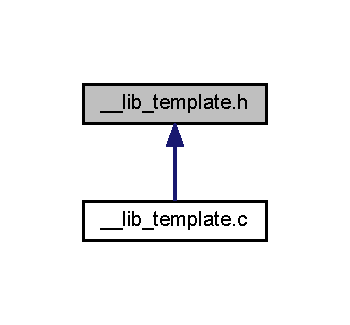
\includegraphics[width=168pt]{____lib__template_8h__dep__incl}
\end{center}
\end{figure}

\section{Commenting Guidelines.\-h File Reference}
\label{_commenting_01_guidelines_8h}\index{Commenting Guidelines.\-h@{Commenting Guidelines.\-h}}
\subsection*{Macros}
\begin{DoxyCompactItemize}
\item 
\#define {\bf \-\_\-\-\_\-\-S\-H\-O\-W\-\_\-\-M\-O\-D\-U\-L\-E\-\_\-\-H\-E\-A\-D\-E\-R\-\_\-\-\_\-}
\begin{DoxyCompactList}\small\item\em This section includes Module Header on the documentation. \end{DoxyCompactList}\item 
\#define {\bf \-\_\-\-\_\-\-P\-H\-\_\-\-C\-O\-M\-M\-E\-N\-T\-S\-\_\-\-\_\-\-H\-\_\-\-\_\-}
\item 
\#define {\bf \-\_\-\-\_\-\-T\-A\-B\-S\-I\-Z\-E}
\item 
\#define {\bf \-\_\-\-\_\-\-F\-O\-N\-T}
\item 
\#define {\bf \-\_\-\-\_\-\-F\-U\-N\-C\-T\-I\-O\-N\-\_\-\-H\-E\-A\-D\-E\-R\-S}
\begin{DoxyCompactList}\small\item\em Function Naming Conventions. \end{DoxyCompactList}\item 
\#define {\bf \-\_\-\-\_\-\-U\-N\-D\-O\-C\-U\-M\-E\-N\-T\-E\-D\-\_\-\-C\-O\-M\-M\-E\-N\-T\-S}
\item 
\#define {\bf \-\_\-\-\_\-\-U\-N\-D\-O\-C\-\_\-\-C\-O\-M\-M\-E\-N\-T\-\_\-\-O\-N\-T\-O\-P}
\item 
\#define {\bf \-\_\-\-\_\-\-U\-N\-D\-O\-C\-\_\-\-C\-O\-M\-M\-E\-N\-T\-\_\-\-A\-F\-T\-E\-R}
\item 
\#define {\bf \-\_\-\-\_\-\-U\-N\-D\-O\-C\-\_\-\-C\-O\-M\-M\-E\-N\-T\-\_\-\-B\-L\-O\-C\-K}
\item 
\#define {\bf \-\_\-\-\_\-\-D\-O\-C\-U\-M\-E\-N\-T\-E\-D\-\_\-\-C\-O\-M\-M\-E\-N\-T\-S}
\begin{DoxyCompactList}\small\item\em Documented Comments on the other hand are comments placed on the code that will be included on the document to be generated by the doxygen. \end{DoxyCompactList}\item 
\#define {\bf \-\_\-\-\_\-\-D\-O\-C\-\_\-\-C\-O\-M\-M\-E\-N\-T\-\_\-\-O\-N\-T\-O\-P}
\begin{DoxyCompactList}\small\item\em This is the Phil\-Robotics standard documented comment that can be placed on top of the members. \end{DoxyCompactList}\item 
\#define {\bf \-\_\-\-\_\-\-D\-O\-C\-\_\-\-C\-O\-M\-M\-E\-N\-T\-\_\-\-A\-F\-T\-E\-R}
\begin{DoxyCompactList}\small\item\em This is the Phil\-Robotics standard documented comment that can be placed after the members. \end{DoxyCompactList}\item 
\#define {\bf \-\_\-\-\_\-\-D\-O\-C\-\_\-\-C\-O\-M\-M\-E\-N\-T\-\_\-\-B\-L\-O\-C\-K}
\begin{DoxyCompactList}\small\item\em This is the Phil\-Robotics standard documented comment block. \end{DoxyCompactList}\item 
\#define {\bf \-\_\-\-\_\-\-D\-O\-C\-\_\-\-B\-R\-I\-E\-F}
\begin{DoxyCompactList}\small\item\em Brief description on comment blocks are shown on function summary of the generated document. The brief description is terminated by an empty line. \end{DoxyCompactList}\item 
\#define {\bf \-\_\-\-\_\-\-D\-O\-C\-\_\-\-P\-A\-R\-A\-G\-R\-A\-P\-H}
\item 
\#define {\bf \-\_\-\-\_\-\-D\-O\-C\-\_\-\-Q\-O\-U\-T\-E\-S}
\item 
\#define {\bf \-\_\-\-\_\-\-D\-O\-C\-\_\-\-E\-M\-P\-H\-A\-S\-I\-Z\-E\-D}
\item 
\#define {\bf \-\_\-\-\_\-\-D\-O\-C\-\_\-\-B\-U\-L\-L\-E\-T\-S}
\item 
\#define {\bf \-\_\-\-\_\-\-D\-O\-C\-\_\-\-L\-I\-N\-K\-S}
\end{DoxyCompactItemize}


\subsection{Macro Definition Documentation}
\index{Commenting Guidelines.\-h@{Commenting Guidelines.\-h}!\-\_\-\-\_\-\-D\-O\-C\-\_\-\-B\-R\-I\-E\-F@{\-\_\-\-\_\-\-D\-O\-C\-\_\-\-B\-R\-I\-E\-F}}
\index{\-\_\-\-\_\-\-D\-O\-C\-\_\-\-B\-R\-I\-E\-F@{\-\_\-\-\_\-\-D\-O\-C\-\_\-\-B\-R\-I\-E\-F}!Commenting Guidelines.h@{Commenting Guidelines.\-h}}
\subsubsection[{\-\_\-\-\_\-\-D\-O\-C\-\_\-\-B\-R\-I\-E\-F}]{\setlength{\rightskip}{0pt plus 5cm}\#define \-\_\-\-\_\-\-D\-O\-C\-\_\-\-B\-R\-I\-E\-F}\label{_commenting_01_guidelines_8h_a5d32347608032efb5f94f60964dc39fc}


Brief description on comment blocks are shown on function summary of the generated document. The brief description is terminated by an empty line. 

After the empty line. A detailed description can follow. 

Definition at line 106 of file Commenting Guidelines.\-h.

\index{Commenting Guidelines.\-h@{Commenting Guidelines.\-h}!\-\_\-\-\_\-\-D\-O\-C\-\_\-\-B\-U\-L\-L\-E\-T\-S@{\-\_\-\-\_\-\-D\-O\-C\-\_\-\-B\-U\-L\-L\-E\-T\-S}}
\index{\-\_\-\-\_\-\-D\-O\-C\-\_\-\-B\-U\-L\-L\-E\-T\-S@{\-\_\-\-\_\-\-D\-O\-C\-\_\-\-B\-U\-L\-L\-E\-T\-S}!Commenting Guidelines.h@{Commenting Guidelines.\-h}}
\subsubsection[{\-\_\-\-\_\-\-D\-O\-C\-\_\-\-B\-U\-L\-L\-E\-T\-S}]{\setlength{\rightskip}{0pt plus 5cm}\#define \-\_\-\-\_\-\-D\-O\-C\-\_\-\-B\-U\-L\-L\-E\-T\-S}\label{_commenting_01_guidelines_8h_ac89283ca91abe3a2207ab2cd854b99fb}


Definition at line 119 of file Commenting Guidelines.\-h.

\index{Commenting Guidelines.\-h@{Commenting Guidelines.\-h}!\-\_\-\-\_\-\-D\-O\-C\-\_\-\-C\-O\-M\-M\-E\-N\-T\-\_\-\-A\-F\-T\-E\-R@{\-\_\-\-\_\-\-D\-O\-C\-\_\-\-C\-O\-M\-M\-E\-N\-T\-\_\-\-A\-F\-T\-E\-R}}
\index{\-\_\-\-\_\-\-D\-O\-C\-\_\-\-C\-O\-M\-M\-E\-N\-T\-\_\-\-A\-F\-T\-E\-R@{\-\_\-\-\_\-\-D\-O\-C\-\_\-\-C\-O\-M\-M\-E\-N\-T\-\_\-\-A\-F\-T\-E\-R}!Commenting Guidelines.h@{Commenting Guidelines.\-h}}
\subsubsection[{\-\_\-\-\_\-\-D\-O\-C\-\_\-\-C\-O\-M\-M\-E\-N\-T\-\_\-\-A\-F\-T\-E\-R}]{\setlength{\rightskip}{0pt plus 5cm}\#define \-\_\-\-\_\-\-D\-O\-C\-\_\-\-C\-O\-M\-M\-E\-N\-T\-\_\-\-A\-F\-T\-E\-R}\label{_commenting_01_guidelines_8h_a05481f633e29eef515b0444498677613}


This is the Phil\-Robotics standard documented comment that can be placed after the members. 



Definition at line 92 of file Commenting Guidelines.\-h.

\index{Commenting Guidelines.\-h@{Commenting Guidelines.\-h}!\-\_\-\-\_\-\-D\-O\-C\-\_\-\-C\-O\-M\-M\-E\-N\-T\-\_\-\-B\-L\-O\-C\-K@{\-\_\-\-\_\-\-D\-O\-C\-\_\-\-C\-O\-M\-M\-E\-N\-T\-\_\-\-B\-L\-O\-C\-K}}
\index{\-\_\-\-\_\-\-D\-O\-C\-\_\-\-C\-O\-M\-M\-E\-N\-T\-\_\-\-B\-L\-O\-C\-K@{\-\_\-\-\_\-\-D\-O\-C\-\_\-\-C\-O\-M\-M\-E\-N\-T\-\_\-\-B\-L\-O\-C\-K}!Commenting Guidelines.h@{Commenting Guidelines.\-h}}
\subsubsection[{\-\_\-\-\_\-\-D\-O\-C\-\_\-\-C\-O\-M\-M\-E\-N\-T\-\_\-\-B\-L\-O\-C\-K}]{\setlength{\rightskip}{0pt plus 5cm}\#define \-\_\-\-\_\-\-D\-O\-C\-\_\-\-C\-O\-M\-M\-E\-N\-T\-\_\-\-B\-L\-O\-C\-K}\label{_commenting_01_guidelines_8h_a67edf61ed8b786078bf4b121f25dfae8}


This is the Phil\-Robotics standard documented comment block. 



Definition at line 98 of file Commenting Guidelines.\-h.

\index{Commenting Guidelines.\-h@{Commenting Guidelines.\-h}!\-\_\-\-\_\-\-D\-O\-C\-\_\-\-C\-O\-M\-M\-E\-N\-T\-\_\-\-O\-N\-T\-O\-P@{\-\_\-\-\_\-\-D\-O\-C\-\_\-\-C\-O\-M\-M\-E\-N\-T\-\_\-\-O\-N\-T\-O\-P}}
\index{\-\_\-\-\_\-\-D\-O\-C\-\_\-\-C\-O\-M\-M\-E\-N\-T\-\_\-\-O\-N\-T\-O\-P@{\-\_\-\-\_\-\-D\-O\-C\-\_\-\-C\-O\-M\-M\-E\-N\-T\-\_\-\-O\-N\-T\-O\-P}!Commenting Guidelines.h@{Commenting Guidelines.\-h}}
\subsubsection[{\-\_\-\-\_\-\-D\-O\-C\-\_\-\-C\-O\-M\-M\-E\-N\-T\-\_\-\-O\-N\-T\-O\-P}]{\setlength{\rightskip}{0pt plus 5cm}\#define \-\_\-\-\_\-\-D\-O\-C\-\_\-\-C\-O\-M\-M\-E\-N\-T\-\_\-\-O\-N\-T\-O\-P}\label{_commenting_01_guidelines_8h_a958480aceeadf39dc04920ba2747ffdb}


This is the Phil\-Robotics standard documented comment that can be placed on top of the members. 



Definition at line 90 of file Commenting Guidelines.\-h.

\index{Commenting Guidelines.\-h@{Commenting Guidelines.\-h}!\-\_\-\-\_\-\-D\-O\-C\-\_\-\-E\-M\-P\-H\-A\-S\-I\-Z\-E\-D@{\-\_\-\-\_\-\-D\-O\-C\-\_\-\-E\-M\-P\-H\-A\-S\-I\-Z\-E\-D}}
\index{\-\_\-\-\_\-\-D\-O\-C\-\_\-\-E\-M\-P\-H\-A\-S\-I\-Z\-E\-D@{\-\_\-\-\_\-\-D\-O\-C\-\_\-\-E\-M\-P\-H\-A\-S\-I\-Z\-E\-D}!Commenting Guidelines.h@{Commenting Guidelines.\-h}}
\subsubsection[{\-\_\-\-\_\-\-D\-O\-C\-\_\-\-E\-M\-P\-H\-A\-S\-I\-Z\-E\-D}]{\setlength{\rightskip}{0pt plus 5cm}\#define \-\_\-\-\_\-\-D\-O\-C\-\_\-\-E\-M\-P\-H\-A\-S\-I\-Z\-E\-D}\label{_commenting_01_guidelines_8h_a8102db00a4cbe5f47b65cfbd81422240}


Definition at line 116 of file Commenting Guidelines.\-h.

\index{Commenting Guidelines.\-h@{Commenting Guidelines.\-h}!\-\_\-\-\_\-\-D\-O\-C\-\_\-\-L\-I\-N\-K\-S@{\-\_\-\-\_\-\-D\-O\-C\-\_\-\-L\-I\-N\-K\-S}}
\index{\-\_\-\-\_\-\-D\-O\-C\-\_\-\-L\-I\-N\-K\-S@{\-\_\-\-\_\-\-D\-O\-C\-\_\-\-L\-I\-N\-K\-S}!Commenting Guidelines.h@{Commenting Guidelines.\-h}}
\subsubsection[{\-\_\-\-\_\-\-D\-O\-C\-\_\-\-L\-I\-N\-K\-S}]{\setlength{\rightskip}{0pt plus 5cm}\#define \-\_\-\-\_\-\-D\-O\-C\-\_\-\-L\-I\-N\-K\-S}\label{_commenting_01_guidelines_8h_a0c8f9e8fcf822f8fff7ff7b0fce3eced}


Definition at line 120 of file Commenting Guidelines.\-h.

\index{Commenting Guidelines.\-h@{Commenting Guidelines.\-h}!\-\_\-\-\_\-\-D\-O\-C\-\_\-\-P\-A\-R\-A\-G\-R\-A\-P\-H@{\-\_\-\-\_\-\-D\-O\-C\-\_\-\-P\-A\-R\-A\-G\-R\-A\-P\-H}}
\index{\-\_\-\-\_\-\-D\-O\-C\-\_\-\-P\-A\-R\-A\-G\-R\-A\-P\-H@{\-\_\-\-\_\-\-D\-O\-C\-\_\-\-P\-A\-R\-A\-G\-R\-A\-P\-H}!Commenting Guidelines.h@{Commenting Guidelines.\-h}}
\subsubsection[{\-\_\-\-\_\-\-D\-O\-C\-\_\-\-P\-A\-R\-A\-G\-R\-A\-P\-H}]{\setlength{\rightskip}{0pt plus 5cm}\#define \-\_\-\-\_\-\-D\-O\-C\-\_\-\-P\-A\-R\-A\-G\-R\-A\-P\-H}\label{_commenting_01_guidelines_8h_a5c18421713f12a583800d00676c6a98d}


Definition at line 108 of file Commenting Guidelines.\-h.

\index{Commenting Guidelines.\-h@{Commenting Guidelines.\-h}!\-\_\-\-\_\-\-D\-O\-C\-\_\-\-Q\-O\-U\-T\-E\-S@{\-\_\-\-\_\-\-D\-O\-C\-\_\-\-Q\-O\-U\-T\-E\-S}}
\index{\-\_\-\-\_\-\-D\-O\-C\-\_\-\-Q\-O\-U\-T\-E\-S@{\-\_\-\-\_\-\-D\-O\-C\-\_\-\-Q\-O\-U\-T\-E\-S}!Commenting Guidelines.h@{Commenting Guidelines.\-h}}
\subsubsection[{\-\_\-\-\_\-\-D\-O\-C\-\_\-\-Q\-O\-U\-T\-E\-S}]{\setlength{\rightskip}{0pt plus 5cm}\#define \-\_\-\-\_\-\-D\-O\-C\-\_\-\-Q\-O\-U\-T\-E\-S}\label{_commenting_01_guidelines_8h_ab32ee8b32058560618cb6c1435e2c7df}
\begin{quotation}
Comment blocks can have a \par
 qoute emphasis \end{quotation}


Definition at line 114 of file Commenting Guidelines.\-h.

\index{Commenting Guidelines.\-h@{Commenting Guidelines.\-h}!\-\_\-\-\_\-\-D\-O\-C\-U\-M\-E\-N\-T\-E\-D\-\_\-\-C\-O\-M\-M\-E\-N\-T\-S@{\-\_\-\-\_\-\-D\-O\-C\-U\-M\-E\-N\-T\-E\-D\-\_\-\-C\-O\-M\-M\-E\-N\-T\-S}}
\index{\-\_\-\-\_\-\-D\-O\-C\-U\-M\-E\-N\-T\-E\-D\-\_\-\-C\-O\-M\-M\-E\-N\-T\-S@{\-\_\-\-\_\-\-D\-O\-C\-U\-M\-E\-N\-T\-E\-D\-\_\-\-C\-O\-M\-M\-E\-N\-T\-S}!Commenting Guidelines.h@{Commenting Guidelines.\-h}}
\subsubsection[{\-\_\-\-\_\-\-D\-O\-C\-U\-M\-E\-N\-T\-E\-D\-\_\-\-C\-O\-M\-M\-E\-N\-T\-S}]{\setlength{\rightskip}{0pt plus 5cm}\#define \-\_\-\-\_\-\-D\-O\-C\-U\-M\-E\-N\-T\-E\-D\-\_\-\-C\-O\-M\-M\-E\-N\-T\-S}\label{_commenting_01_guidelines_8h_a99e6a732bbd43c67e56c23a9246bdc1d}


Documented Comments on the other hand are comments placed on the code that will be included on the document to be generated by the doxygen. 



Definition at line 87 of file Commenting Guidelines.\-h.

\index{Commenting Guidelines.\-h@{Commenting Guidelines.\-h}!\-\_\-\-\_\-\-F\-O\-N\-T@{\-\_\-\-\_\-\-F\-O\-N\-T}}
\index{\-\_\-\-\_\-\-F\-O\-N\-T@{\-\_\-\-\_\-\-F\-O\-N\-T}!Commenting Guidelines.h@{Commenting Guidelines.\-h}}
\subsubsection[{\-\_\-\-\_\-\-F\-O\-N\-T}]{\setlength{\rightskip}{0pt plus 5cm}\#define \-\_\-\-\_\-\-F\-O\-N\-T}\label{_commenting_01_guidelines_8h_a09cb312bd214bc572375aa86aab440a4}
font shall be courier or any equally spaced font 

Definition at line 53 of file Commenting Guidelines.\-h.

\index{Commenting Guidelines.\-h@{Commenting Guidelines.\-h}!\-\_\-\-\_\-\-F\-U\-N\-C\-T\-I\-O\-N\-\_\-\-H\-E\-A\-D\-E\-R\-S@{\-\_\-\-\_\-\-F\-U\-N\-C\-T\-I\-O\-N\-\_\-\-H\-E\-A\-D\-E\-R\-S}}
\index{\-\_\-\-\_\-\-F\-U\-N\-C\-T\-I\-O\-N\-\_\-\-H\-E\-A\-D\-E\-R\-S@{\-\_\-\-\_\-\-F\-U\-N\-C\-T\-I\-O\-N\-\_\-\-H\-E\-A\-D\-E\-R\-S}!Commenting Guidelines.h@{Commenting Guidelines.\-h}}
\subsubsection[{\-\_\-\-\_\-\-F\-U\-N\-C\-T\-I\-O\-N\-\_\-\-H\-E\-A\-D\-E\-R\-S}]{\setlength{\rightskip}{0pt plus 5cm}\#define \-\_\-\-\_\-\-F\-U\-N\-C\-T\-I\-O\-N\-\_\-\-H\-E\-A\-D\-E\-R\-S}\label{_commenting_01_guidelines_8h_ac4b5df0c06e000352574229919103b4a}


Function Naming Conventions. 


\begin{DoxyItemize}
\item must be as short as possible (2-\/4 words long)
\item function names must follow the format [action][Module][Parameter]
\begin{DoxyItemize}
\item e.\-g. get\-Pin\-Value(\-Pin)
\end{DoxyItemize}
\item the [Parameter] may be omitted if there are no parameters to be set or derived on the module
\begin{DoxyItemize}
\item e.\-g. set\-Pin(\-Pin), clr\-Pin(\-Pin)
\end{DoxyItemize}
\item the [Module] may be omitted if the [Parameter] is exclusive to the module or for the purpose of simplicity
\begin{DoxyItemize}
\item e.\-g. get\-M\-S() 
\end{DoxyItemize}
\end{DoxyItemize}

Definition at line 70 of file Commenting Guidelines.\-h.

\index{Commenting Guidelines.\-h@{Commenting Guidelines.\-h}!\-\_\-\-\_\-\-P\-H\-\_\-\-C\-O\-M\-M\-E\-N\-T\-S\-\_\-\-\_\-\-H\-\_\-\-\_\-@{\-\_\-\-\_\-\-P\-H\-\_\-\-C\-O\-M\-M\-E\-N\-T\-S\-\_\-\-\_\-\-H\-\_\-\-\_\-}}
\index{\-\_\-\-\_\-\-P\-H\-\_\-\-C\-O\-M\-M\-E\-N\-T\-S\-\_\-\-\_\-\-H\-\_\-\-\_\-@{\-\_\-\-\_\-\-P\-H\-\_\-\-C\-O\-M\-M\-E\-N\-T\-S\-\_\-\-\_\-\-H\-\_\-\-\_\-}!Commenting Guidelines.h@{Commenting Guidelines.\-h}}
\subsubsection[{\-\_\-\-\_\-\-P\-H\-\_\-\-C\-O\-M\-M\-E\-N\-T\-S\-\_\-\-\_\-\-H\-\_\-\-\_\-}]{\setlength{\rightskip}{0pt plus 5cm}\#define \-\_\-\-\_\-\-P\-H\-\_\-\-C\-O\-M\-M\-E\-N\-T\-S\-\_\-\-\_\-\-H\-\_\-\-\_\-}\label{_commenting_01_guidelines_8h_a9775ef95daddfe5e2f6dfc499769c6d8}


Definition at line 36 of file Commenting Guidelines.\-h.

\index{Commenting Guidelines.\-h@{Commenting Guidelines.\-h}!\-\_\-\-\_\-\-S\-H\-O\-W\-\_\-\-M\-O\-D\-U\-L\-E\-\_\-\-H\-E\-A\-D\-E\-R\-\_\-\-\_\-@{\-\_\-\-\_\-\-S\-H\-O\-W\-\_\-\-M\-O\-D\-U\-L\-E\-\_\-\-H\-E\-A\-D\-E\-R\-\_\-\-\_\-}}
\index{\-\_\-\-\_\-\-S\-H\-O\-W\-\_\-\-M\-O\-D\-U\-L\-E\-\_\-\-H\-E\-A\-D\-E\-R\-\_\-\-\_\-@{\-\_\-\-\_\-\-S\-H\-O\-W\-\_\-\-M\-O\-D\-U\-L\-E\-\_\-\-H\-E\-A\-D\-E\-R\-\_\-\-\_\-}!Commenting Guidelines.h@{Commenting Guidelines.\-h}}
\subsubsection[{\-\_\-\-\_\-\-S\-H\-O\-W\-\_\-\-M\-O\-D\-U\-L\-E\-\_\-\-H\-E\-A\-D\-E\-R\-\_\-\-\_\-}]{\setlength{\rightskip}{0pt plus 5cm}\#define \-\_\-\-\_\-\-S\-H\-O\-W\-\_\-\-M\-O\-D\-U\-L\-E\-\_\-\-H\-E\-A\-D\-E\-R\-\_\-\-\_\-}\label{_commenting_01_guidelines_8h_aa61948e995c04179b19d5e2ad6f5ac9f}


This section includes Module Header on the documentation. 

\subsection*{Phil\-Robotics $|$ Philippine Electronics and Robotics Enthusiasts Club}

{\tt http\-://philrobotics.\-com} $|$ {\tt http\-://philrobotics.\-com/forum} $|$ {\tt http\-://facebook.\-com/philrobotics} {\tt phirobotics.\-core@philrobotics.\-com} 

 \begin{TabularC}{2}
\hline
\rowcolor{lightgray}{\bf Filename\-: }&{\bf \char`\"{}\-Commenting Guidelines.\-h\char`\"{} }\\\cline{1-2}
Description\-: &This serves as a guide on how to place comments on the code for Phil\-Robotics projects \\\cline{1-2}
Revision\-: &vxx.\-xx.\-xx \\\cline{1-2}
Author\-: &[author's name] \\\cline{1-2}
&\\\cline{1-2}
Dependencies\-: &\\\cline{1-2}
\end{TabularC}


\begin{quotation}
This program is free software\-: you can redistribute it and/or modify it under the terms of the G\-N\-U General Public License as published by the Free Software Foundation, either version 3 of the License, or (at your option) any later version. This program is distributed in the hope that it will be useful, but W\-I\-T\-H\-O\-U\-T A\-N\-Y W\-A\-R\-R\-A\-N\-T\-Y; without even the implied warranty of M\-E\-R\-C\-H\-A\-N\-T\-A\-B\-I\-L\-I\-T\-Y or F\-I\-T\-N\-E\-S\-S F\-O\-R A P\-A\-R\-T\-I\-C\-U\-L\-A\-R P\-U\-R\-P\-O\-S\-E. See the G\-N\-U General Public License for more details. \par
\par
 You should have received a copy of the G\-N\-U General Public License along with this program. If not, see {\tt http\-://www.\-gnu.\-org/licenses/}

\end{quotation}
\subsubsection*{\par
}

\begin{TabularC}{4}
\hline
\rowcolor{lightgray}{\bf F\-W Version }&{\bf Date }&{\bf Author }&{\bf Description }\\\cline{1-4}
vxx.\-xx.\-xx &Y\-Y\-Y\-Y\-M\-M\-D\-D &[author's name] &Library Initial Release \\\cline{1-4}
\end{TabularC}


Definition at line 32 of file Commenting Guidelines.\-h.

\index{Commenting Guidelines.\-h@{Commenting Guidelines.\-h}!\-\_\-\-\_\-\-T\-A\-B\-S\-I\-Z\-E@{\-\_\-\-\_\-\-T\-A\-B\-S\-I\-Z\-E}}
\index{\-\_\-\-\_\-\-T\-A\-B\-S\-I\-Z\-E@{\-\_\-\-\_\-\-T\-A\-B\-S\-I\-Z\-E}!Commenting Guidelines.h@{Commenting Guidelines.\-h}}
\subsubsection[{\-\_\-\-\_\-\-T\-A\-B\-S\-I\-Z\-E}]{\setlength{\rightskip}{0pt plus 5cm}\#define \-\_\-\-\_\-\-T\-A\-B\-S\-I\-Z\-E}\label{_commenting_01_guidelines_8h_a92becee03c19eb792bea3841c2cab633}
tab settings shall be 4 characters long and must be represented by spaces 

Definition at line 50 of file Commenting Guidelines.\-h.

\index{Commenting Guidelines.\-h@{Commenting Guidelines.\-h}!\-\_\-\-\_\-\-U\-N\-D\-O\-C\-\_\-\-C\-O\-M\-M\-E\-N\-T\-\_\-\-A\-F\-T\-E\-R@{\-\_\-\-\_\-\-U\-N\-D\-O\-C\-\_\-\-C\-O\-M\-M\-E\-N\-T\-\_\-\-A\-F\-T\-E\-R}}
\index{\-\_\-\-\_\-\-U\-N\-D\-O\-C\-\_\-\-C\-O\-M\-M\-E\-N\-T\-\_\-\-A\-F\-T\-E\-R@{\-\_\-\-\_\-\-U\-N\-D\-O\-C\-\_\-\-C\-O\-M\-M\-E\-N\-T\-\_\-\-A\-F\-T\-E\-R}!Commenting Guidelines.h@{Commenting Guidelines.\-h}}
\subsubsection[{\-\_\-\-\_\-\-U\-N\-D\-O\-C\-\_\-\-C\-O\-M\-M\-E\-N\-T\-\_\-\-A\-F\-T\-E\-R}]{\setlength{\rightskip}{0pt plus 5cm}\#define \-\_\-\-\_\-\-U\-N\-D\-O\-C\-\_\-\-C\-O\-M\-M\-E\-N\-T\-\_\-\-A\-F\-T\-E\-R}\label{_commenting_01_guidelines_8h_a8fc77337a2a32ae81cd1946cce324554}


Definition at line 78 of file Commenting Guidelines.\-h.

\index{Commenting Guidelines.\-h@{Commenting Guidelines.\-h}!\-\_\-\-\_\-\-U\-N\-D\-O\-C\-\_\-\-C\-O\-M\-M\-E\-N\-T\-\_\-\-B\-L\-O\-C\-K@{\-\_\-\-\_\-\-U\-N\-D\-O\-C\-\_\-\-C\-O\-M\-M\-E\-N\-T\-\_\-\-B\-L\-O\-C\-K}}
\index{\-\_\-\-\_\-\-U\-N\-D\-O\-C\-\_\-\-C\-O\-M\-M\-E\-N\-T\-\_\-\-B\-L\-O\-C\-K@{\-\_\-\-\_\-\-U\-N\-D\-O\-C\-\_\-\-C\-O\-M\-M\-E\-N\-T\-\_\-\-B\-L\-O\-C\-K}!Commenting Guidelines.h@{Commenting Guidelines.\-h}}
\subsubsection[{\-\_\-\-\_\-\-U\-N\-D\-O\-C\-\_\-\-C\-O\-M\-M\-E\-N\-T\-\_\-\-B\-L\-O\-C\-K}]{\setlength{\rightskip}{0pt plus 5cm}\#define \-\_\-\-\_\-\-U\-N\-D\-O\-C\-\_\-\-C\-O\-M\-M\-E\-N\-T\-\_\-\-B\-L\-O\-C\-K}\label{_commenting_01_guidelines_8h_a250deeda134747bca6afcb07e417386d}


Definition at line 84 of file Commenting Guidelines.\-h.

\index{Commenting Guidelines.\-h@{Commenting Guidelines.\-h}!\-\_\-\-\_\-\-U\-N\-D\-O\-C\-\_\-\-C\-O\-M\-M\-E\-N\-T\-\_\-\-O\-N\-T\-O\-P@{\-\_\-\-\_\-\-U\-N\-D\-O\-C\-\_\-\-C\-O\-M\-M\-E\-N\-T\-\_\-\-O\-N\-T\-O\-P}}
\index{\-\_\-\-\_\-\-U\-N\-D\-O\-C\-\_\-\-C\-O\-M\-M\-E\-N\-T\-\_\-\-O\-N\-T\-O\-P@{\-\_\-\-\_\-\-U\-N\-D\-O\-C\-\_\-\-C\-O\-M\-M\-E\-N\-T\-\_\-\-O\-N\-T\-O\-P}!Commenting Guidelines.h@{Commenting Guidelines.\-h}}
\subsubsection[{\-\_\-\-\_\-\-U\-N\-D\-O\-C\-\_\-\-C\-O\-M\-M\-E\-N\-T\-\_\-\-O\-N\-T\-O\-P}]{\setlength{\rightskip}{0pt plus 5cm}\#define \-\_\-\-\_\-\-U\-N\-D\-O\-C\-\_\-\-C\-O\-M\-M\-E\-N\-T\-\_\-\-O\-N\-T\-O\-P}\label{_commenting_01_guidelines_8h_a9d34bd0e40f9f1da18c9987ced225a0a}


Definition at line 76 of file Commenting Guidelines.\-h.

\index{Commenting Guidelines.\-h@{Commenting Guidelines.\-h}!\-\_\-\-\_\-\-U\-N\-D\-O\-C\-U\-M\-E\-N\-T\-E\-D\-\_\-\-C\-O\-M\-M\-E\-N\-T\-S@{\-\_\-\-\_\-\-U\-N\-D\-O\-C\-U\-M\-E\-N\-T\-E\-D\-\_\-\-C\-O\-M\-M\-E\-N\-T\-S}}
\index{\-\_\-\-\_\-\-U\-N\-D\-O\-C\-U\-M\-E\-N\-T\-E\-D\-\_\-\-C\-O\-M\-M\-E\-N\-T\-S@{\-\_\-\-\_\-\-U\-N\-D\-O\-C\-U\-M\-E\-N\-T\-E\-D\-\_\-\-C\-O\-M\-M\-E\-N\-T\-S}!Commenting Guidelines.h@{Commenting Guidelines.\-h}}
\subsubsection[{\-\_\-\-\_\-\-U\-N\-D\-O\-C\-U\-M\-E\-N\-T\-E\-D\-\_\-\-C\-O\-M\-M\-E\-N\-T\-S}]{\setlength{\rightskip}{0pt plus 5cm}\#define \-\_\-\-\_\-\-U\-N\-D\-O\-C\-U\-M\-E\-N\-T\-E\-D\-\_\-\-C\-O\-M\-M\-E\-N\-T\-S}\label{_commenting_01_guidelines_8h_a4be95810703ad22687ae778f55e87a62}


Definition at line 73 of file Commenting Guidelines.\-h.


\printindex
\end{document}
